To illustrate the problem of the cross-domain optimization, let us consider an example, created using the NEXMark~\cite{TODO} benchmark model simulating an online auction.

The first query is analytics written on SQL.
It calculates the number of participants for each auction.
\begin{lstlisting}[language=SQL]
SELECT auction.id, COUNT(person) FROM bid
INNER JOIN person ON bidder = person.id
INNER JOIN auction ON auction = auction.id
GROUP BY auction.id
\end{lstlisting}

It is important to detect frauds on online auctions.
So we have an execution graph that computes metric of  probability that the particular bid is fraud.
This metric can be computed in different ways:
only using bids with low latency and low precision
or
also using an information about bidder and auction with bigger latency and better precision.
Thus, an optimal execution graph shape depends on the business requirements of latency that can be placed into the cost-model.

\begin{figure}[h!]
    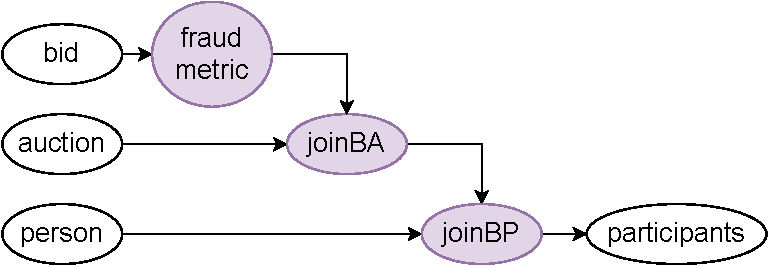
\includegraphics[width=\linewidth]{images/poster.pdf}
    \caption{General execution graph for running example. Purple nodes can be permuted to get an optimal graph.}
    \label{fig}
\end{figure}
